%!TeX program = xelatex
\documentclass[12pt,hyperref,a4paper,UTF8]{ctexart}
\usepackage{SJTUReport}
\usepackage{float}

%%-------------------------------正文开始---------------------------%%
\begin{document}

%%-----------------------封面--------------------%%
\cover

%%------------------摘要-------------%%
%\begin{abstract}
%
%在此填写摘要内容
%
%\end{abstract}

\thispagestyle{empty} % 首页不显示页码

%%--------------------------目录页------------------------%%
\newpage
\tableofcontents

%%------------------------正文页从这里开始-------------------%
\newpage

%%可选择这里也放一个标题
%\begin{center}
%    \title{ \Huge \textbf{{标题}}}
%\end{center}

\section{实验目的}

\begin{enumerate}
    \item 掌握液体沸点的测定方法。
    \item 用热分析法测绘锡-铋二组分体系液固平衡相图。
    \item 掌握热分析法的测量二组分体系液固平衡相图技术。
\end{enumerate}

\section{实验原理}
热分析法是测绘二组分体系液固平衡相图的方法之一。所谓热分析法是将二组分体系的混合物加热熔化成均匀相,然后使体系缓慢冷却,每隔一定时间测定体系的温度,作温度对时间的关系图,所得曲线称为冷却曲线,如图2.5.1所示。当熔融体系在均匀冷却过程中无相变化时,由于热损失的原因,体系的温度将连续均匀下降,实验得到一段光滑的冷却曲线,如图(3)中ab线段;如果体系在冷却过程中发生了相变,则相变热可使热损失有所抵偿,冷却曲线就会出现转折,转折点温度所对应的温度,即为体系的相变温度,如图(3)中b点;体系继续冷却到低共熔混合物的固体析出,如图(3)中c点。在低共熔混合物全部凝固以前,体系温度保持不变。因此冷却曲线上出现水平线段(平台),如图(3)中cd线段;当熔液完全凝固后,温度才迅速下降,如图(3)中de线段。对简单的固相完全不互熔的二组分体系,选择不同组成的体系,则可得类似图(4)(a)所示的冷却曲线,由冷却曲线的转折点可绘出二组分体系液固平衡相图,如图(4)(b)。
\begin{figure}[htp]
    \centering
    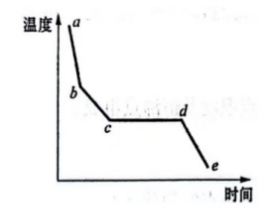
\includegraphics[width=0.5\linewidth]{截屏2023-12-22 21.52.49.png}
    \caption{冷却曲线示意图}
    \label{fig:enter-label3}
\end{figure}


\begin{figure}[htp]
\centering
\subfigure[步冷曲线]{
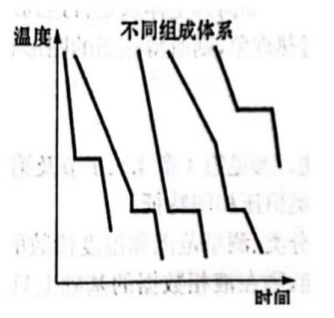
\includegraphics[width=7cm,height =5cm]{截屏2023-12-22 21.56.20.png}}
\subfigure[相图]{
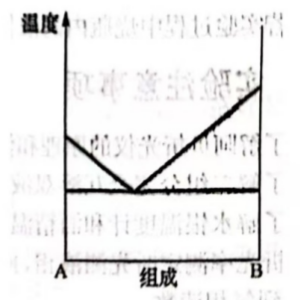
\includegraphics[width=7cm,height =5cm]{截屏2023-12-22 21.57.55.png}}
\caption{简单低共熔二组分体系的冷却曲线和相图}
\label{1}
\end{figure}

用热分析法测绘相图的要点:
\begin{itemize}
    \item 由于相图表示体系达相平衡时的状态,因此冷却速率必须足够慢,以保证被测体系处于或非常接近相平衡状态。
\item 测定过程中应保证样品均匀且无氧化、变质等现象,否则被测体系的组成与原来配制样品时的组成不一致。
\item 测温元件的热容必须足够小,它与被测体系的热传导必须足够良好,以保证测得的温度值能真正反映体系的温度。
\end{itemize}

简单的二组分体系金属相图主要分为液相完全互溶、固相也能完全互溶的体系,如Cu-Ni体系;液相完全互溶、固相完全不互溶的体系,如Cd-Bi体系;液相完全互溶、固相部分互溶的体系,如本实验研究的Sn-Bi体系。在低共熔温度下,Bi在固相Sn中的最大溶解度以质量分数表示为$\omega _B=0.21$。因此,用本实验的方法还不能作出完整的相图。

本实验用铂电阻温度计作测温元件。实验装置如图(5)所示。
\begin{figure}[htp]
    \centering
    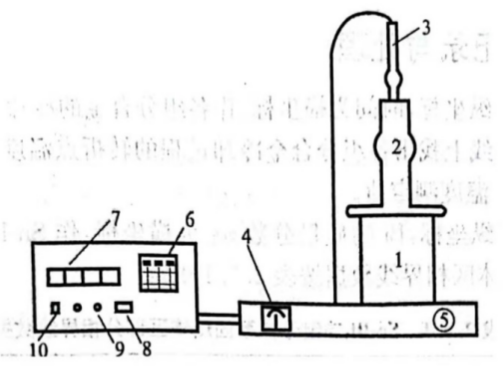
\includegraphics[width=0.5\linewidth]{仪器.png}
    \caption{二组分体系液固相图测定装置图}
    \label{fig:enter-label5}
\end{figure}

1-金属相图炉,2-不锈钢样品管(共6管),3-铂电阻温度计,4-电压表,5-电压调节旋钮,6-温度设置,7-数字显示,8-复位键,9-加热指示灯,10-定时键


\section{实验试剂与仪器}
\subsection{二组分体系气液平衡相图测定实验仪器}
\begin{itemize}
    \item JX-6DS型金属相图炉与微机温度控制仪各1台,其中金属相图炉与实验原理中所示的相图测定装置相似,而微机温度控制仪有所不同,本实验所用仪器面板如下图所示。
    \begin{figure}[htp]
        \centering
        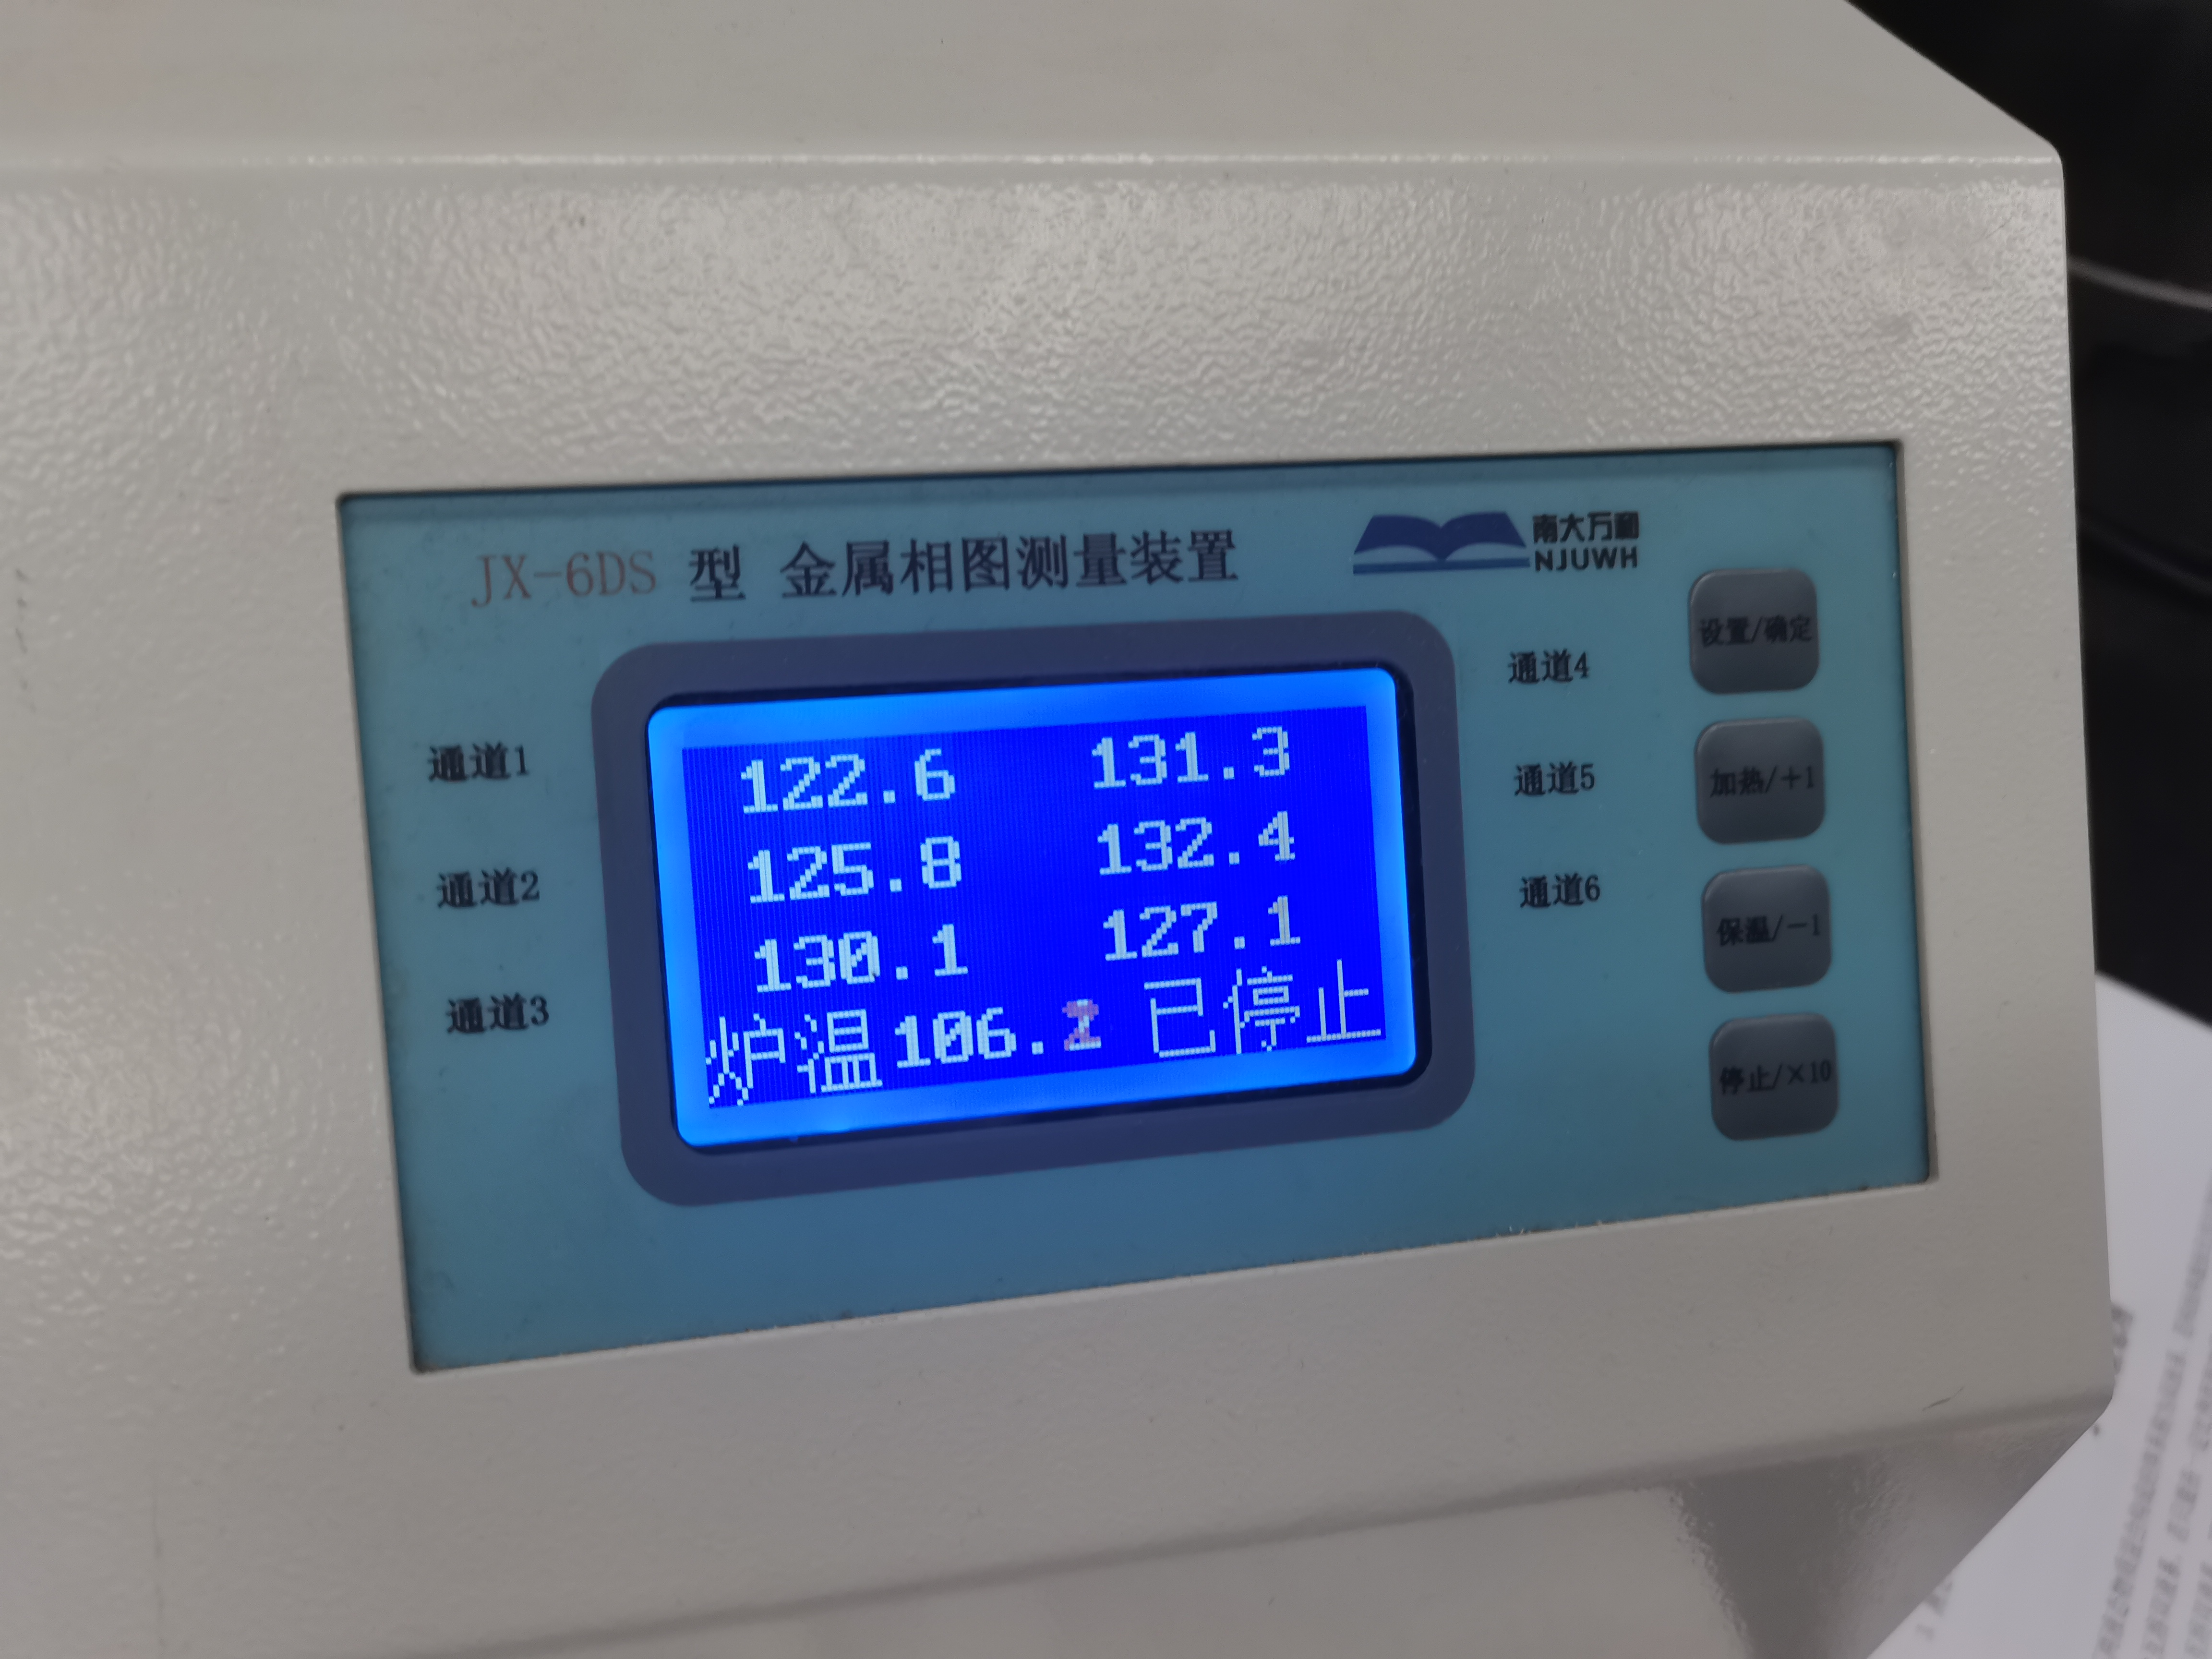
\includegraphics[width=0.5\linewidth]{WechatIMG631.jpg}
        \caption{微机温度控制仪操作面板示意图}
        \label{fig:enter-label7}
    \end{figure}
    \item 铂电阻温度计1支
    \item 不锈钢样品管6支
    
\end{itemize}

\subsection{二组分体系液固平衡相图测定实验试剂}
纯锡,纯铋,石墨粉

\section{实验步骤}

\begin{enumerate}
    \item \textbf{配制样品}:
    用感量为0.1g的托盘天平分别配制含铋质量分数为0.30、0,40、0.58和0.80的铋锡混合物各100g,纯铋、纯锡各100g,将样品分别放人不锈钢样品管中,上面覆盖一层石墨粉。具体实验中该步骤已预先完成。
    \item \textbf{样品测定}:
    \begin{itemize}
        \item 接通电源,在微电脑温度控制仪上,根据不同样品通过温度设置键设置不同的加热温度(一般控制在样品完全熔化后再上升$30^{\circ}C$左右),本实验调节加热温度为$350^{\circ}C$,按下确认键,此时加热指示灯亮,样品己开始加热。
        \item 将装有金属或合金的样品管放入金属相图炉中加热,使之熔化,将铂电阻温度计插入样品管中,控制温度计顶部离样品管底部约1cm。
        \item 当体系温度超过设置温度后,金属相图炉自动停止加热。摁下停止键,系统开始降温。每分钟记录一次六通道中的熔化温度。测定直至温度降至约$100^{\circ}C$时停止实验。
    \end{itemize}
    \item \textbf{数据记录与处理}
    \begin{itemize}
        \item 以温度为纵坐标,时间为横坐标,作各组分合金的冷却曲线。
        \item 在冷却曲线上找出各组分合金冷却过程的转折点温度。根据纯Bi、纯Sn的熔点校正转折点温度测定值。
        \item 以温度为纵坐标,Bi的质量分数$\omega_{Bi}$为横坐标,作Sn-Bi二组分体系液固相图。其Sn固溶体区相界线数据按下表确定。
        \begin{table}[htp]
        \centering
        \caption{Sn-Bi二组分体系固熔体区部分相界线数据}
\begin{tabular}{|l|l|l|l|l|l|l|l|l|l|l|}
\hline
$\omega_{Bi}$ & 0.05 & 0.10 & 0.15 & 0.21  & 0.158 & 0.116 & 0.082 & 0.053 & 0.027 & 0.01 \\ \hline
温度t$/^{\circ}C$ & 210  & 185  & 162  & 低共熔 & 120   & 100   & 80    & 60    & 40    & 20   \\ \hline
\end{tabular}
\end{table}
    \end{itemize}
\end{enumerate}

\clearpage

\section{实验数据记录}

\subsection{原始数据}
数据量较大,具体数据见附表。

\subsection{步冷曲线}
\begin{figure}[H]
    \
    \centering
    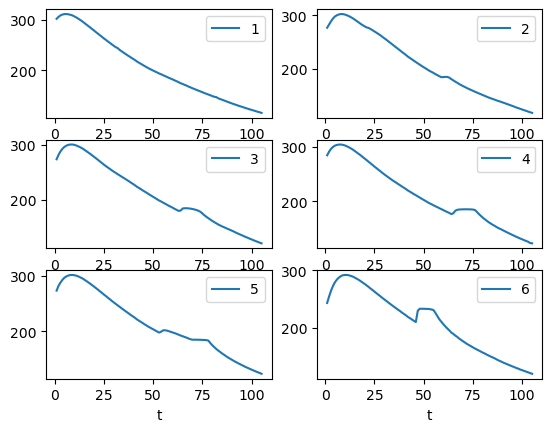
\includegraphics[width=0.8\linewidth]{f1.png}
    \caption{各个通道中的T-t图像}
    \label{fig:enter-label6}
\end{figure}



\section{数据处理}
\subsection{步冷曲线}
\begin{figure}[H]
\centering
\subfigure[6条步冷曲线集合]{
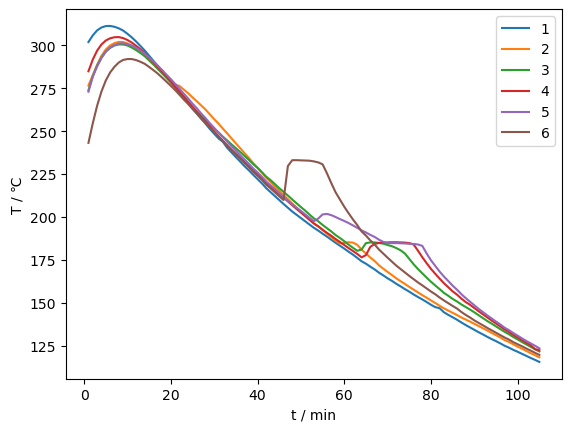
\includegraphics[width=7cm,height =6cm]{f2.png}}
\subfigure[6条步冷曲线离散]{
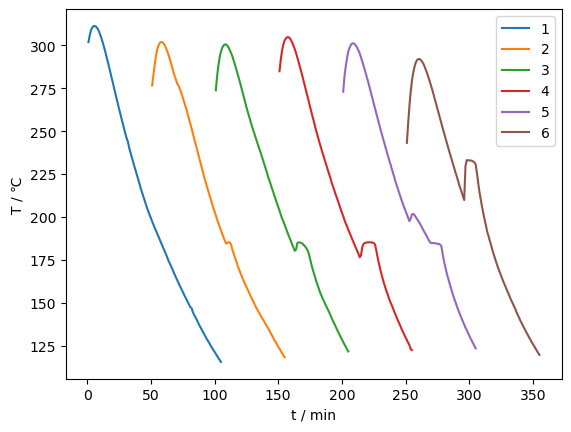
\includegraphics[width=7cm,height =6cm]{f3.png}}
\end{figure}


\subsection{转折温度与相图}
\begin{table}[htp]
\centering
\caption{各通道溶解温度}
\begin{tabular}{|l|l|l|l|l|l|l|}
\hline
$\omega _{Bi}$     & 0.00  & 0.30  & 0.40  & 0.58  & 0.80  & 1.00  \\ \hline
第一转折点$/^{\circ}C$ & 237.6 & 272.1 & 234.6 & 185.2 & 205.8 & 232.9 \\ \hline
第二转折点$/^{\circ}C$ &       & 185.1 & 185.2 & 185.2 & 184.8 & 185.0 \\ \hline
\end{tabular}
\end{table}


\begin{figure}[H]
    \centering
    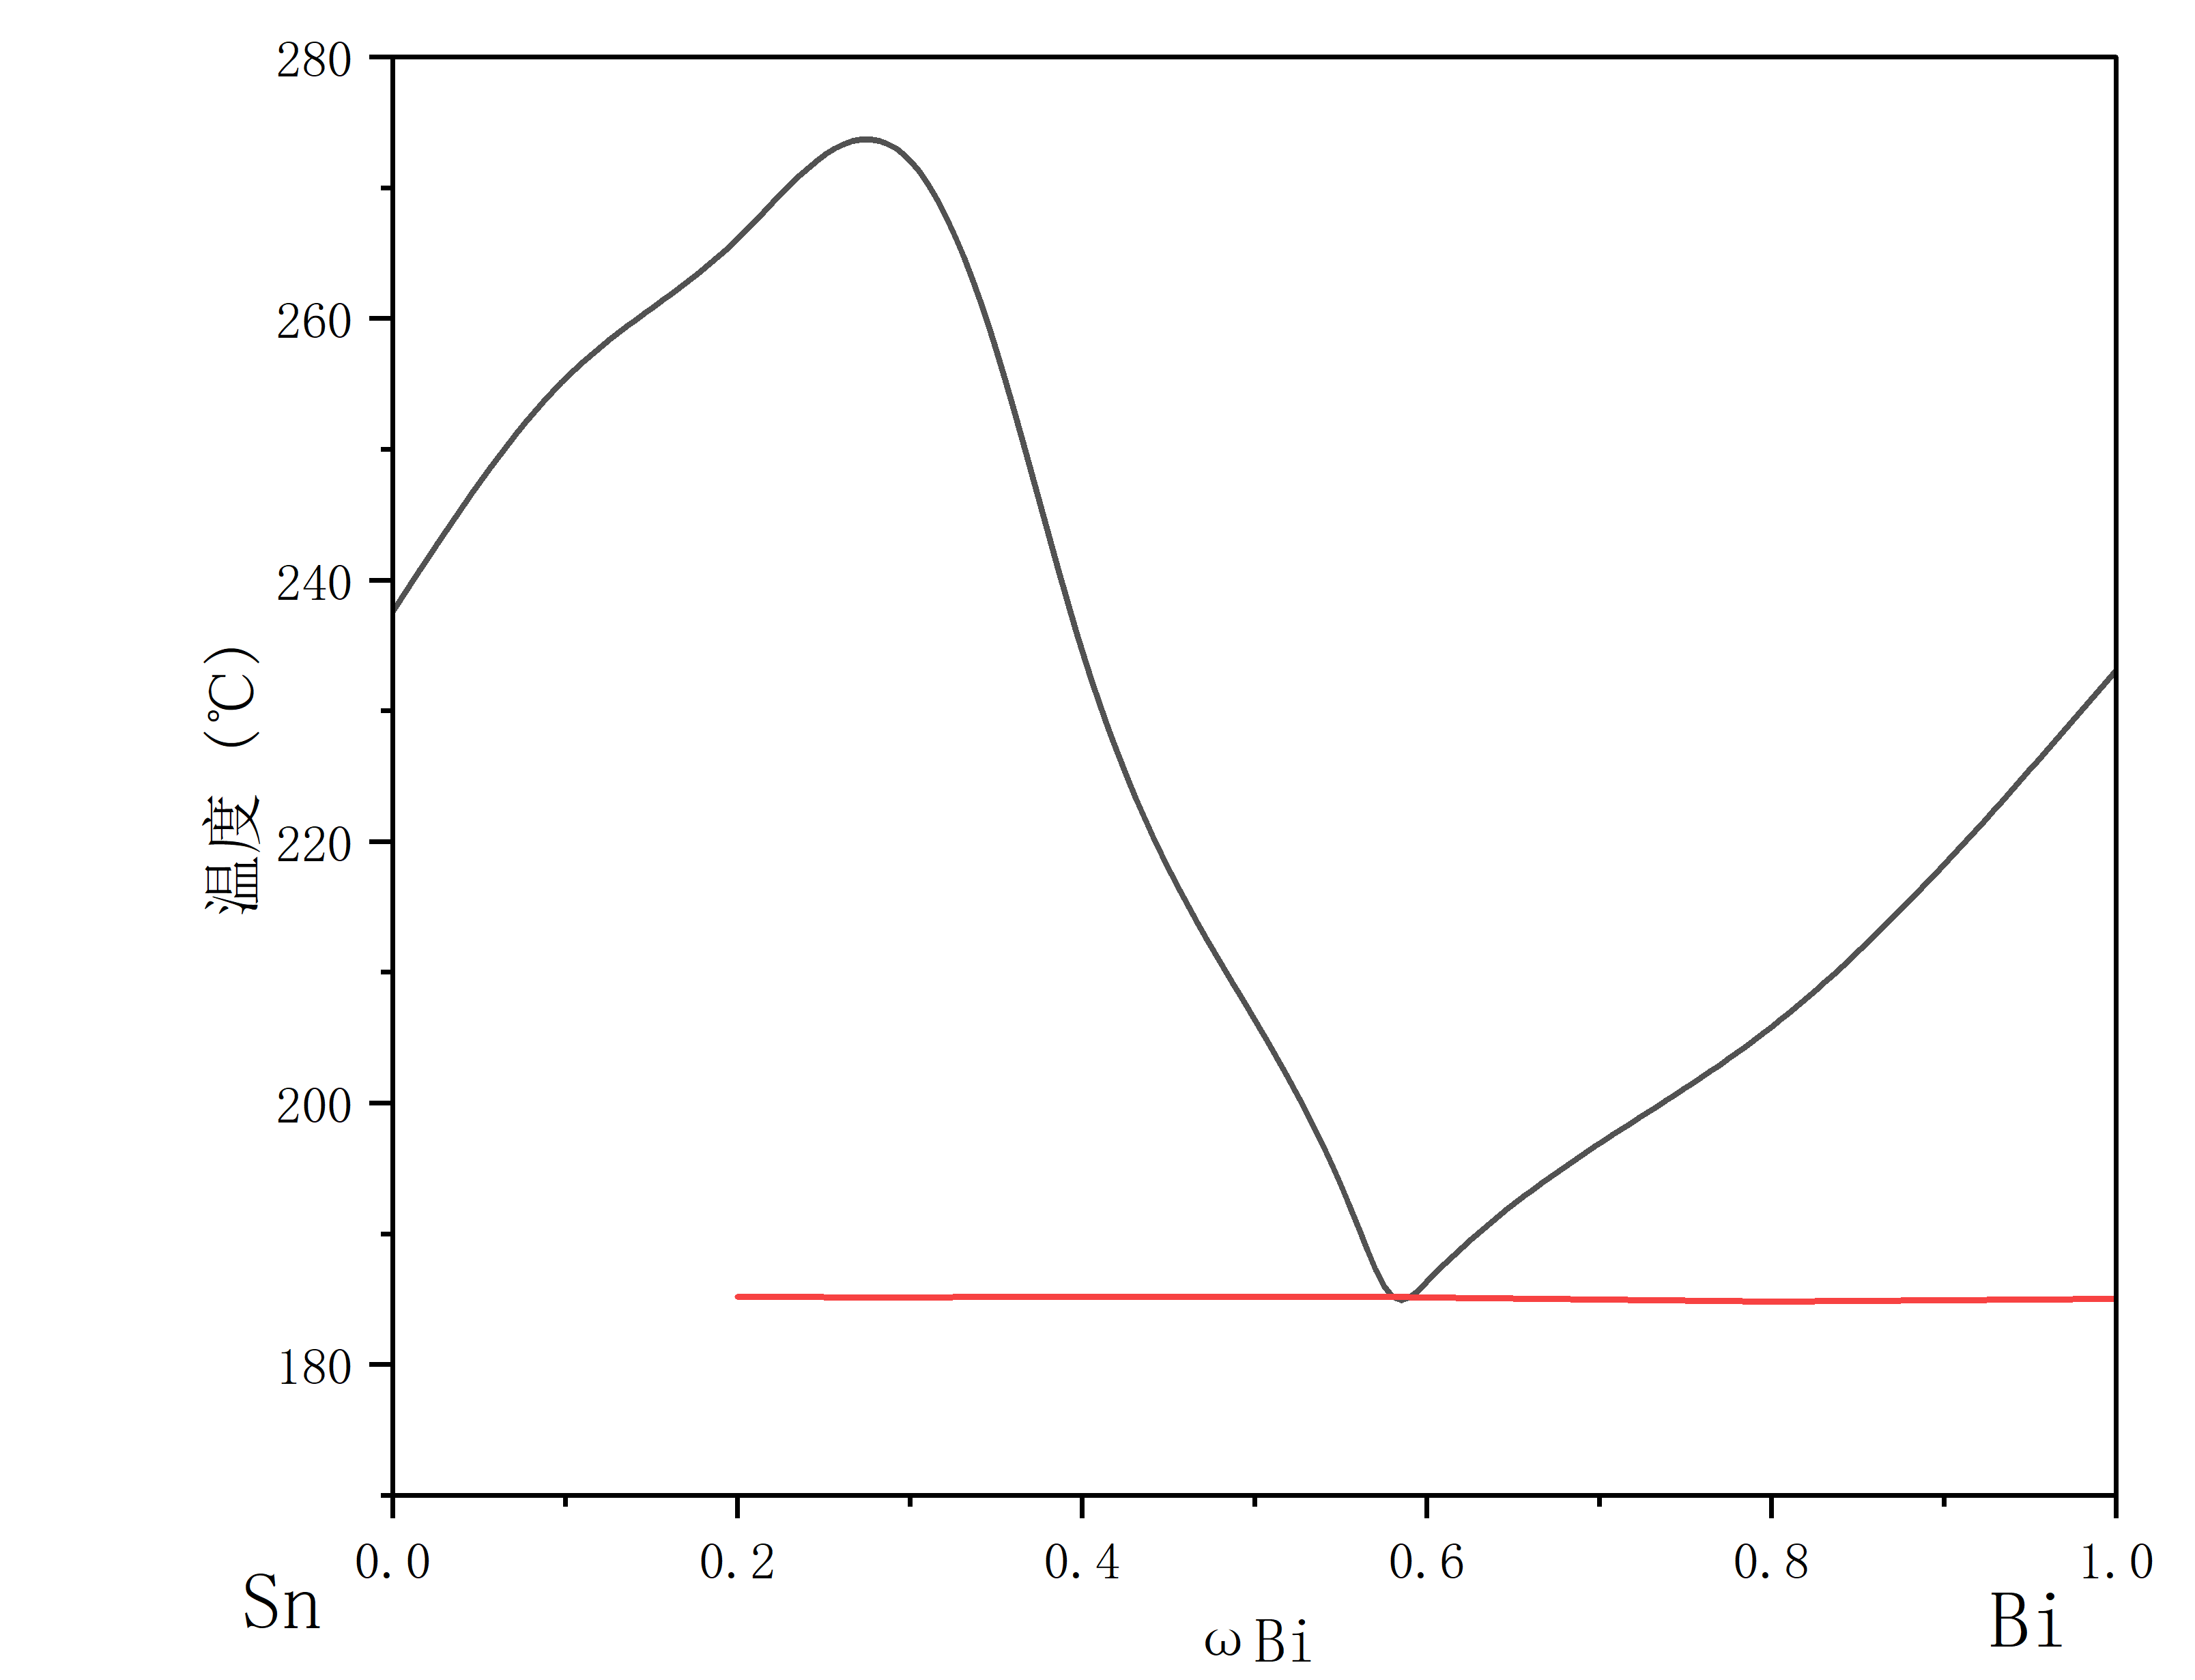
\includegraphics[width=0.7\linewidth]{WechatIMG636.jpg}
    \caption{Sn-Bi相图}
    \label{fig:enter-label8}
\end{figure}

\clearpage

\section{数据分析与讨论}
\subsection{结果分析}
根据本实验测得的Sn-Bi相图以及理论情况中的Sn-Bi相图\cite{1}(如下图所示),经过深入讨论与分析,得出以下结论:
\begin{figure}[H]
    \centering
    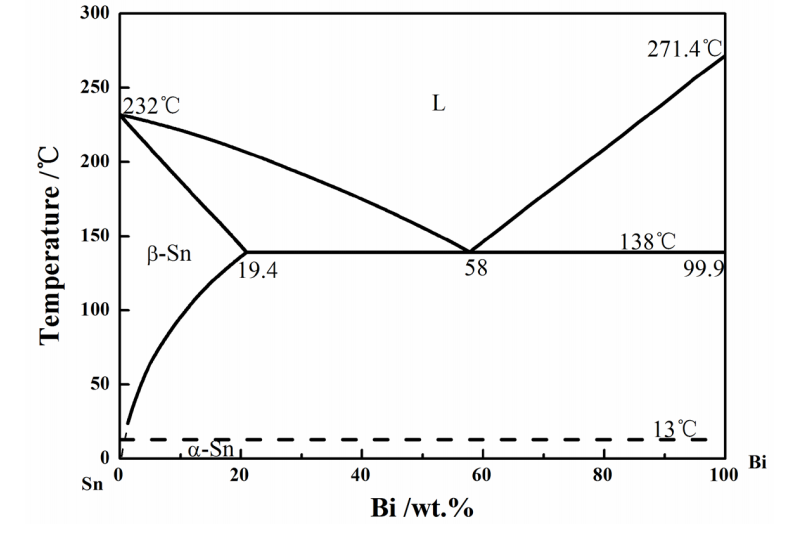
\includegraphics[width=0.5\linewidth]{截屏2023-12-23 11.32.52.png}
    \caption{Sn-Bi理论相图示意图}
    \label{fig:enter-label12}
\end{figure}
实验初期获得的冷却曲线呈现出意想不到的上升趋势。理想情况下,冷却曲线应该从一开始就呈下降趋势,以反映熔融样品温度的持续下降。上升趋势表明,在计时开始时,样品管中的所有固体并没有完全熔化,仍在吸收热量。为了解决这个问题,建议在开始实验前稍微超过目标温度,以确保样品完全熔化。

测得纯锡的熔点为 $237.6^{\circ}C$ 。外部数据表明纯锡的熔点为 $232.0^{\circ}C$ \cite{1},因此相对误差为 2.41\%。纯铋的熔点为 $232.9^{\circ}C$ ,而文献建议的熔点为 $271.4^{\circ}C$ \cite{1},由此产生了 14.18\% 的显著相对误差。测量值偏低的原因可能是铋样品中含有杂质,可能包括铟或其他金属杂质。锡铋体系的共晶点记录为 $185.2^{\circ}C$ ,大大高于报告的共晶温度 $138.0^{\circ}C$ \cite{1},相对误差超过 30\%。造成这种差异的潜在原因包括:
\begin{enumerate}
    \item 铋的纯度不够,导致二元混合物不理想,影响共晶温度。
    \item 实验温度控制不完善,且Bi的熔点较高,导致样品在开始时没有完全熔化,影响了相变温度测量的准确性。
    \item 实验测量的相图在 $\omega _{Bi} = 0.30$ 处出现异常突起。可以推测,这表明形成了一种高熔点化合物。为了确定化合物的成分和化学式,应测量铋质量分数在 0.30 左右的二元体系的冷却曲线。然而,由于电负性和原子结构的差异,锡和铋在正常条件下不会形成稳定的化合物,这表明杂质可能会影响高熔点化合物的形成。
    \item 测量设备出现延迟问题,可能会影响温度测量的准确性。
    \item  一些测得的冷却曲线,如通道 (2) 中的曲线,没有明显的拐点。这可能意味着金属析出量相对较少,拐点可能与杂质析出相对应,导致锡析出时斜率变化不明显。
\end{enumerate}



\section{思考题}
   
\subsection{绘制二组分相图常用哪些方法?}
    
构建二元相图的常用方法包括热分析法(动态法)和淬火法(静态法),其中热分析法又分为冷却曲线法和差热分析法(DSC)。DSC 通过测量样品在加热或冷却过程中吸收或释放的热量来确定相变温度。淬火法包括观察合金在不同温度和成分下固相和液相的相对比例。光学显微镜可通过分析显微镜下样品的光学特性(包括液相点、固相点和共晶点)来确定相变。X 射线衍射 (XRD) 可以分析合金的晶体结构,确定晶格参数并深入了解相变。
    
\subsection{试用相律分析各冷却曲线上出现平台何转折点的原因。}
    
在熔融金属体系的冷却过程中,当熔体中某一成分达到饱和状态时,纯金属晶体开始析出。金属凝固的放热反应补偿了系统的热量损失,减缓了冷却速度,导致冷却曲线的斜率发生变化,从而出现拐点。
    
\subsection{ 为什么在不同组分的熔融液的冷却曲线上,最低共熔点的水平线段长度不同?}
    
    最低共熔点指的是混合物在冷却过程中从液态向固态转变的温度最低的点。这个转变过程并非瞬间完成,而是在一定的温度范围内发生的。不同组分的混合物在冷却过程中的相变温度范围可能不同,且析出的共熔物组分总量不同,因此最低共熔点的水平线段长度也就不同。
    
\subsection{ 若已知二组分体系的许多不同组成的冷曲线,但不知道低共熔点组成,有什么办法确定?}
先对步冷曲线进行分析,在所有已知冷却曲线中,寻找具有明显水平平台(即温度保持不变阶段)的曲线,这通常表明发生了相变过程,在此过程中,温度会在某一固定值上停留,直到所有液体转变为固态。
共熔点附近的冷却曲线会显示出最长的水平平台,因为在共熔温度下,液态混合物将开始凝固,直到所有的液体都固化成固态共熔组成,这个过程需要释放大量的热。

再通过绘制相图进一步判断,将所有冷却曲线的数据点(特别是开始凝固和结束凝固的温度)绘制在温度-组成(T-C)图上。通过连接相同相变过程中的数据点,可以描绘出液相线和固相线。液相线和固相线的交点即为共熔点。



\clearpage

\section{附表}
\begin{table}[htp]
\centering
\caption{二组分体系液固平衡相图的测定原始数据}
\begin{tabular}{|l|l|l|l|l|l|l|}
\hline
时间/min & 通道1/°C & 通道2/°C & 通道3/°C & 通道4/°C & 通道5/°C & 通道6/°C \\ \hline
1      & 301.9  & 276.6  & 273.8  & 284.9  & 273    & 243.2  \\ \hline
2      & 305.8  & 282.7  & 281.9  & 291.7  & 281.8  & 254.6  \\ \hline
3      & 308.7  & 288.7  & 288.2  & 296.9  & 287.7  & 264.8  \\ \hline
4      & 310.4  & 293.9  & 292.9  & 300.5  & 292.6  & 273.1  \\ \hline
5      & 311.2  & 297.6  & 296.3  & 302.8  & 296.3  & 279.5  \\ \hline
6      & 311.3  & 299.9  & 298.5  & 304.1  & 298.7  & 284.2  \\ \hline
7      & 310.8  & 301.3  & 299.9  & 304.7  & 300.2  & 287.5  \\ \hline
8      & 309.9  & 302    & 300.5  & 304.8  & 301.1  & 290    \\ \hline
9      & 308.6  & 301.9  & 300.5  & 304.2  & 301.2  & 291.5  \\ \hline
10     & 306.7  & 301.1  & 299.9  & 303.1  & 300.7  & 292    \\ \hline
11     & 304.6  & 299.8  & 298.7  & 301.6  & 299.9  & 292    \\ \hline
12     & 302.2  & 298.2  & 297.2  & 299.7  & 298.6  & 291.4  \\ \hline
13     & 299.6  & 296.3  & 295.5  & 297.7  & 296.9  & 290.4  \\ \hline
14     & 296.9  & 294.2  & 293.6  & 295.5  & 295.2  & 289.2  \\ \hline
15     & 293.9  & 291.7  & 291.2  & 292.9  & 292.9  & 287.4  \\ \hline
16     & 290.9  & 289.1  & 288.8  & 290.2  & 290.6  & 285.5  \\ \hline
17     & 287.9  & 286.5  & 286.2  & 287.5  & 288.1  & 283.5  \\ \hline
18     & 284.9  & 283.8  & 283.7  & 284.8  & 285.6  & 281.2  \\ \hline
19     & 281.7  & 281.4  & 281    & 281.9  & 282.9  & 278.8  \\ \hline
20     & 278.7  & 279.3  & 278.3  & 279    & 280.3  & 276.4  \\ \hline
21     & 275.5  & 277.2  & 275.5  & 276.1  & 277.5  & 273.9  \\ \hline
22     & 272.4  & 276.3  & 272.7  & 273.1  & 274.7  & 271.2  \\ \hline
23     & 269.3  & 274.2  & 269.8  & 270.2  & 271.8  & 268.4  \\ \hline
24     & 266.3  & 272.1  & 267    & 267.2  & 269    & 265.8  \\ \hline
25     & 263.1  & 269.7  & 264.1  & 264.1  & 266    & 263    \\ \hline
26     & 260.2  & 267.4  & 261.4  & 261.3  & 263.3  & 260.3  \\ \hline








\end{tabular}
\end{table}

\begin{table}[htp]
\centering
\begin{tabular}{|l|l|l|l|l|l|l|}
\hline
时间/min & 通道1/°C & 通道2/°C & 通道3/°C & 通道4/°C & 通道5/°C & 通道6/°C \\ \hline
27     & 257.2  & 265    & 258.9  & 258.3  & 260.3  & 257.5  \\ \hline
28     & 254.4  & 262.6  & 256.4  & 255.6  & 257.6  & 254.9  \\ \hline
29     & 251.3  & 259.8  & 253.8  & 252.5  & 254.6  & 252    \\ \hline
30     & 248.5  & 257    & 251.4  & 249.8  & 251.9  & 249.4  \\ \hline
31     & 245.8  & 254.4  & 249.2  & 247.1  & 249.2  & 246.8  \\ \hline
32     & 243.8  & 251.5  & 246.8  & 244.4  & 246.5  & 244.1  \\ \hline
33     & 240.3  & 248.7  & 244.6  & 241.8  & 243.9  & 241.5  \\ \hline
34     & 237.6  & 245.8  & 242.3  & 239.2  & 241.2  & 238.9  \\ \hline
35     & 234.9  & 242.9  & 240.1  & 236.8  & 238.6  & 236.4  \\ \hline
36     & 232.3  & 240.1  & 237.9  & 234.5  & 236    & 233.9  \\ \hline
37     & 229.6  & 237.2  & 235.6  & 232    & 233.5  & 231.4  \\ \hline
38     & 227.2  & 234.4  & 233.3  & 229.7  & 231    & 229    \\ \hline
39     & 224.6  & 231.4  & 230.8  & 227.2  & 228.3  & 226.3  \\ \hline
40     & 222.1  & 228.7  & 228.6  & 224.9  & 226    & 224    \\ \hline
41     & 219.6  & 225.9  & 226.1  & 222.6  & 223.5  & 221.6  \\ \hline
42     & 216.8  & 222.8  & 223.5  & 219.9  & 220.7  & 218.8  \\ \hline
43     & 214.5  & 220.4  & 221.5  & 217.8  & 218.5  & 216.7  \\ \hline
44     & 212.2  & 217.8  & 219.2  & 215.6  & 216.3  & 214.4  \\ \hline
45     & 209.9  & 215.3  & 216.8  & 213.3  & 213.9  & 212.1  \\ \hline
46     & 207.6  & 212.8  & 214.7  & 211.3  & 211.7  & 209.9  \\ \hline
47     & 205.4  & 210.4  & 212.5  & 209.1  & 209.4  & 229.7  \\ \hline
48     & 203.2  & 207.9  & 210.2  & 206.9  & 207.4  & 233.1  \\ \hline
49     & 201.3  & 205.5  & 208    & 204.7  & 205.4  & 233.1  \\ \hline
50     & 199.4  & 203.2  & 205.8  & 202.6  & 203.5  & 233    \\ \hline
51     & 197.5  & 201    & 203.7  & 200.5  & 201.5  & 232.9  \\ \hline
52     & 195.6  & 198.6  & 201.4  & 198.3  & 199.5  & 232.8  \\ \hline
53     & 193.7  & 196.3  & 199.2  & 196.2  & 197.6  & 232.4  \\ \hline
54     & 192.1  & 194.5  & 197.5  & 194.6  & 199.1  & 231.8  \\ \hline
55     & 190.3  & 192.4  & 195.4  & 192.6  & 201.5  & 230.7  \\ \hline
56     & 188.6  & 190.3  & 193.5  & 190.8  & 201.8  & 225.5  \\ \hline
57     & 186.8  & 188.3  & 191.6  & 189.1  & 201.1  & 219.8  \\ \hline
58     & 185    & 186.3  & 189.5  & 187.2  & 200    & 214.4  \\ \hline
59     & 183.3  & 184.6  & 187.8  & 185.5  & 198.8  & 210.2  \\ \hline
60     & 181.6  & 184.9  & 185.9  & 183.7  & 197.7  & 206    \\ \hline
\end{tabular}
\end{table}


\begin{table}[htp]
\centering
\begin{tabular}{|l|l|l|l|l|l|l|}
\hline
时间/min & 通道1/°C & 通道2/°C & 通道3/°C & 通道4/°C & 通道5/°C & 通道6/°C \\ \hline
61     & 179.8  & 185.3  & 183.9  & 181.9  & 196.5  & 202.2  \\ \hline
62     & 178.1  & 185.1  & 182.1  & 180.2  & 195.1  & 198.6  \\ \hline
63     & 176.2  & 183.8  & 180.3  & 178.5  & 193.7  & 195.3  \\ \hline
64     & 174.2  & 181    & 181.1  & 176.5  & 192.2  & 191.6  \\ \hline
65     & 172.8  & 178.8  & 184.8  & 177.8  & 191    & 189.2  \\ \hline
66     & 171.1  & 176.4  & 185.2  & 182.6  & 189.6  & 186.4  \\ \hline
67     & 169.5  & 174.4  & 185.2  & 184.3  & 188.4  & 184    \\ \hline
68     & 167.6  & 171.9  & 184.9  & 184.9  & 186.8  & 181.1  \\ \hline
69     & 166    & 169.9  & 184.5  & 185.1  & 185.5  & 178.7  \\ \hline
70     & 164.3  & 168    & 183.7  & 185.2  & 184.8  & 176.3  \\ \hline
71     & 162.8  & 166.2  & 183    & 185.3  & 184.8  & 174    \\ \hline
72     & 161.1  & 164.3  & 181.9  & 185.3  & 184.8  & 171.7  \\ \hline
73     & 159.6  & 162.6  & 180.6  & 185.2  & 184.7  & 169.7  \\ \hline
74     & 158    & 161    & 178.7  & 185.1  & 184.6  & 167.7  \\ \hline
75     & 156.5  & 159.3  & 175.6  & 184.8  & 184.4  & 165.7  \\ \hline
76     & 154.9  & 157.7  & 172.5  & 184    & 184.3  & 163.8  \\ \hline
77     & 153.4  & 156.1  & 169.7  & 180.4  & 184    & 161.9  \\ \hline
78     & 152    & 154.5  & 167.2  & 176.6  & 183.2  & 160.2  \\ \hline
79     & 150.5  & 153    & 164.7  & 173.1  & 178.8  & 158.4  \\ \hline
80     & 148.9  & 151.4  & 162.3  & 169.8  & 174.8  & 156.6  \\ \hline
81     & 147.5  & 149.9  & 160.1  & 166.9  & 171.5  & 155    \\ \hline
82     & 146.9  & 148.3  & 158    & 164.1  & 168.2  & 153.1  \\ \hline
83     & 144.5  & 146.8  & 155.8  & 161.4  & 165.3  & 151.4  \\ \hline
84     & 143    & 145.5  & 154.1  & 159.1  & 162.7  & 149.8  \\ \hline
85     & 141.6  & 144.2  & 152.3  & 156.7  & 160    & 148.2  \\ \hline
86     & 140.2  & 142.9  & 150.8  & 154.8  & 157.7  & 146.7  \\ \hline
87     & 138.6  & 141.5  & 149.1  & 152.5  & 155.1  & 144.7  \\ \hline
88     & 137.1  & 140.3  & 147.6  & 150.5  & 152.8  & 143    \\ \hline
89     & 135.7  & 139.1  & 146.1  & 148.9  & 150.7  & 141.5  \\ \hline
90     & 134.3  & 137.8  & 144.5  & 147    & 148.6  & 139.8  \\ \hline
91     & 132.9  & 136.5  & 142.8  & 145.1  & 146.5  & 138.3  \\ \hline
92     & 131.6  & 135.2  & 141.1  & 143.3  & 144.6  & 136.9  \\ \hline
93     & 130.2  & 133.9  & 139.4  & 141.5  & 142.7  & 135.4  \\ \hline
94     & 128.9  & 132.5  & 137.9  & 139.7  & 140.9  & 134    \\ \hline
\end{tabular}
\end{table}

\begin{table}
\centering
\begin{tabular}{|l|l|l|l|l|l|l|}
\hline
时间/min & 通道1/°C & 通道2/°C & 通道3/°C & 通道4/°C & 通道5/°C & 通道6/°C \\ \hline
95     & 127.7  & 131.2  & 136.3  & 138    & 139.1  & 132.6  \\ \hline
96     & 126.4  & 129.8  & 134.7  & 136.3  & 137.4  & 131.2  \\ \hline
97     & 125    & 128.3  & 133.1  & 134.5  & 135.5  & 129.8  \\ \hline
98     & 123.9  & 127.2  & 131.7  & 133    & 134.1  & 128.6  \\ \hline
99     & 122.6  & 125.8  & 130.1  & 131.3  & 132.4  & 127.1  \\ \hline
100    & 121.5  & 124.5  & 128.7  & 129.9  & 130.9  & 125.9  \\ \hline
101    & 120.3  & 123.3  & 127.2  & 128.3  & 129.3  & 124.7  \\ \hline
102    & 119.1  & 122    & 125.8  & 126.8  & 127.8  & 123.4  \\ \hline
103    & 117.9  & 120.7  & 124.4  & 125.4  & 126.4  & 122.2  \\ \hline
104    & 116.8  & 119.5  & 123    & 123    & 125    & 120.9  \\ \hline
105    & 115.6  & 118.3  & 121.7  & 122.5  & 123.5  & 119.7  \\ \hline
\end{tabular}
\end{table}


\clearpage

%%----------- 参考文献 -------------------%%
%在reference.bib文件中填写参考文献,此处自动生成


\reference

\end{document}